\documentclass[pdftex, a4paper, 11pt]{article}
\usepackage[english]{babel}
\usepackage{fancyhdr,graphicx}
\usepackage[hmargin=2cm,vmargin=2cm,a4paper]{geometry}
\usepackage{hyperref}

\pagestyle{fancy}
\lhead{\scshape Curriculum Vitae (IN PROGRESS AND TRANSLATION)}
\rhead{\itshape Enrico Carlesso}
\rfoot{\footnotesize pag. \thepage}
\cfoot{}
\lfoot{{\footnotesize Updated at:} \today}
\renewcommand{\headrulewidth}{1pt}
\renewcommand{\footrulewidth}{1pt}

\begin{document}
\vspace*{.3cm}
\begin{center}
  \rule{.8\textwidth}{1pt}\\[10pt]
  \begin{minipage}{.55\textwidth}
    \LARGE\textbf{Enrico Carlesso}\\[13pt]
    \small Via Julia, 37\\
    36060 - Romano d'Ezzelino (VI)\\[6pt]
    \textbf{e-mail: enrico@ecarlesso.org}\\
    \small \url{http://www.ecarlesso.org}\\
    \small Phone: 348 858 77 86\\[6pt]
    %% \small Data di nascita: 03.12.1984\\
  \end{minipage}
  \begin{minipage}{.2\textwidth}
    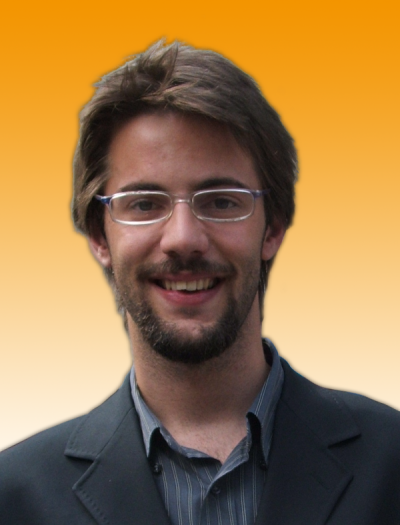
\includegraphics[width=\textwidth]{foto.png}
  \end{minipage}\\[5pt]
  \rule{.8\textwidth}{1pt}
\end{center}
\vspace*{1cm}

\section*{Current Position:}

\hspace{0.58cm}Approaching the degree in Computer Engineering at ``Universit\`a degli Studi di Padova''. 

Stageaire in R\&D division of M31.

% Iscrizione al Registro Imprese con Partita IVA
% n. 03472460249 con qualifica di ``Consulente nel settore delle
% tecnologie dell'informatica''


\section*{Teaching}
\begin{itemize}
\item Bachelor degree in Computer Engineering - 92/110 (Universit\`a degli studi di Padova, 2007);
\item Accounting Diploma (I.T.C.G. L. Einaudi di Bassano del Grappa, 2003).
\end{itemize}

\section*{Experiences}
\begin{itemize}
\item Full-time stage in R\&D di M31 focused on webservice development and new technologies;
\item Web application for different customers;
\item Consultant for server design, deploy and maintenance;
\item German Open 2007, ``Humanoids Legue'' with team from Universit\`a
degli Studi di Padova;
\item Thesis care of Intelligent Autonomous Systems Laboratory titled ``Simultaneous
algorithms of localization and mapping based on Computer Vision'';
\item Some opensource software written, mostly in Python and C.
\end{itemize}

\section*{Computer skills}
\begin{description}
\item[S.O.:] GNU/Linux, Archlinux \& Slackware {\em as first}, deep knowledge
  in every field, from installation, to configuration, to support-software
  writing. Deep knowledge of {\em bash} scripting and good ability in scripting.
  Deep knowledge in server area.
\item[Programming:] Excellent knowkedge of Python and C. Experience in programming
  with many other languages (Ruby, Java, Perl, C++);
\item[Python:] Deep knowledge in programming and dedicated environment: pyOpenGL,
  OpenCV bindings, pyQT. Deep knowledge of Twisted Framework. Knowledge of pys60
  for Symbian;
\item[Web:] Excellent knowledge of PHP, MYSQL e PostgreSQL, deep experience in 
  everything web-related. Deep knowledge of CakePHP, Django and Ruby on Rails frameworks,
  and basic knowledge of important python minor frameworks (cherrypy, web.py, ...). Deep
  knowledge in Javascript, mostly in Mootools and jQuery library;
\item[Electronics:] Good knowledge in Atmel microcontroller programming. Basic experience
  in PCB design. Knowledge of Eagle program. Development of a control board for robot
  engines control;
\item[Other:] \LaTeX, emacs, (py)QT, OpenGL, vim, iptables, cups,
  samba, foss, network management.
\end{description}

\section*{Working Experience}
\begin{itemize}
\item April 2010/Now: Stageaire at M31;
\item May 2008/Now: freelance;
\item January/May 2008: hardware/software care at DV Service (Romano d'Ezzelino - VI - Italy);
\item May/October 2007: Research and develompent at Zilio
  S.p.A. (Cassola - VI - Italy), design and sell of a linux-based video surveillance
  system with HD cameras;
\item 1999/2004: Week-end waiter at Villa Razzolini Loredan (Asolo - TV - Italy);
\item June/October 2002: Technical clerk at ``IALC'' (Romano d'Ezzelino - VI - Italy).
\end{itemize}

% \section*{Active Projects}
% \begin{itemize}
% \item pynokia: program which send sms (and some other interaction)
%   over a bluetooth/cable connection to a Nokia phone. {\em (Python)}\\
% \item videntify: program which gets information from video files. {\em (C)}\\
% %  \url{http://www.ecarlesso.org/works/show/videntify}
% % \item Freesky: scheda controllo motori da servomodellismo,
% %   progettazione, assemblamento e firmware. {\em (Eagle, ARM-C)}\\
% %  \url{http://www.ecarlesso.org/index.php/freesky}
% \end{itemize}

%% \section*{Portfolio WEB}
%% \begin{description}
%% \item[cnssrl.it] Sito dell'azienda CNS srl, con catalogo prodotti
%%   e backend di amministrazione a misura del cliente. Basato su CakePHP
%%   e MooTools\\
%%   \url{http://www.cnssrl.it};
%% \item[ecarlesso.org] Sito personale, in continua crescita. Basato
%%   su CakePhP e MooTools\\
%%   \url{http://www.ecarlesso.org};
%% \end{description}

\section*{Peronal interest}
\begin{itemize}
\item Computer science;
\item {\bf F}ree and {\bf O}pen {\bf S}ource {\bf S}oftware;
\item Math, with special interest in algebra;
\item Interaction between Electronic end Informatic;
\item October 2009 - Now: Linux User Group of Bassano del Grappa (GrappaLUG).
\end{itemize}

\section*{Language skills}
\begin{description}
\item[Italian:] Mother tongue;
\item[English:] Good level of understanding and writing;
\item[German:] Basic knowledge.
\end{description}


\vfill

%% Ai sensi della legge 675/96 (tutela della persona ed altri soggetti
%% rispetto al trattamento dei dati personali), autorizzo al trattamento
%% dei dati personali contenuti nel presente Curriculum Vitae per
%% permettere un adeguata valutazione della mia candidatura finalizzata all'assunzione.
I authorize to deal with information in this document according to the Italian Law n. 675/96

\vspace{1cm}

\footnotesize {This resume is under {\em git}. You can checkout the updated version:}
\begin{verbatim}
    $ git clone git://github.com/carlesso/ecarlesso_cv.git
\end{verbatim}
\end{document}
